\documentclass[a4paper,12pt]{article} 
\usepackage[T2A]{fontenc}			
\usepackage[utf8]{inputenc}			
\usepackage[english,russian]{babel}
\usepackage{float}
\usepackage{amsmath,amsfonts,amssymb,amsthm,mathrsfs,mathtools} 
\usepackage{cancel}
\usepackage{multirow}
\usepackage[colorlinks, linkcolor = blue]{hyperref}
\usepackage{upgreek}\usepackage[left=2cm,right=2cm,top=2cm,bottom=3cm,bindingoffset=0cm]{geometry}
\usepackage{tikz}
\usepackage{graphicx}
\usepackage{subfig}
\usepackage{titletoc}
\usepackage{pgfplots}
\usepackage{xcolor}
\usepackage{wrapfig}
\usepackage{pgfplots}
\pgfplotsset{width=10cm,compat=1.9}

\begin{document}

\begin{titlepage}
		\vspace*{\fill}
		
		\begin{center}
			
\includegraphics[scale=0.8]{MIPT.pdf}
			\\[0.7cm]\Huge Московский Физико-Технический Институт
			\\[2cm]\LARGE Отчет по эксперименту
			\\[0.5cm]\noindent\rule{\textwidth}{1pt}
			\\\Huge\textbf{4.3.1.\\ Изучение дифракции света}
			\\[-0.5cm]\noindent\rule{\textwidth}{1pt}
		\end{center}
		
		\vspace*{\fill}
		
		\begin{flushleft}
			Выполнила: \hspace{\fill} Группа:
			\\Малиновская София \hspace{\fill} Б05-102
		\end{flushleft}
	\end{titlepage}

	\setcounter{page}{2}


\section*{Цель работы} 
Исследовать явления дифракции Френеля и Фраунгофера на щели, изучить влияние дифракции на разрешающую способность оптических инструментов.


\section*{В работе используются}
Оптическая скамья, ртутная лампа, монохроматор, щели с регулируемой шириной, рамка с вертикальной нитью, двойная щель, микроскоп на поперечных салазках с микрометрическим винтом, зрительная труба.


\section*{Теоретическая сводка}
\paragraph{Дифракция Френеля}
Суммарное ширина $n$ зон Френеля $z_n$ определяется соотношением 
\begin{equation}
    z_n = \sqrt{an\lambda}
\end{equation}
где $n$ -- номер зоны, $a$ -- расстояние от щели до плоскости наьлюдений, $\lambda$ -- длина волны. В работе используется ртутная лампа с длиной волны $\lambda = 5461 \cdot 10^{-10}$ м.

\paragraph{Дифракция Фрауегофера}
При дифракции Фраунгофера на одной щели имеет место соотношение
\begin{equation}
    X_m = f_2 m \frac{\lambda}{D}
\end{equation}
где $X_m$ -- расстояние темной полосы от оптическое оси объектива, $f_2$ -- фокусное расстояние линзы, $m$ -- номер темной полосы, $D$ -- ширина щели. \\
При дифракции Фраунгофера на двух щелях будем пользоваться соотношением 
\begin{equation}
    \delta x = f_2 \frac{\lambda}{d} = \frac{2d}{Dn}
\end{equation}
где $\delta x$ -- линейное расстояние между соседними интерференционными полосами в плоскости наблюдения, $n$ -- число темных полос в центральном максимуме.

\paragraph{Влияние дифракции на разрешающую способность оптических приборов} при исследовании влияния дифракции на разрешающую способность оптических систем будем пользоваться соотношеним 
\begin{equation}
    \frac{\lambda}{D_0} = \frac{l}{f_2} = \frac{d}{f_1}
\end{equation}
где $D_0$ -- ширина щели, при которых изображения обеих щелей едва различимы, $f_1$ -- фокусное расстояние, $l$ -- расстояние между изображениями двух щелей.


\section*{Ход работы}
\paragraph{Дифракция Френеля} соберем схему согласно рис. 1. Световые лучи освещают щель $ S_2 $ и испытывают на ней дифракцию. Дифракционная картина рассматривается с помощью микроскопа М, сфокусированного на некоторую плоскость наблюдения П. Щель $ S_2 $ освещается параллельным пучком монохроматического света с помощью коллиматора, образованного объективом $ O_1 $, и щелью $S_1$, находящейся в его фокусе. На щель $ S_1 $ сфокусировано изображение спектральной линии, выделенной из спектра ртутной лампы Л при помощи простого монохроматора C, в котором используется призма прямого зрения. Распределение интенсивности света в плоскости наблюдения П проще всего рассчитывать с помощью зон Френеля. Настроим установку так, чтобы в микроскоп наблюдалась картина дифракции Френеля (пример на рис. 2).

\begin{figure}[H]
    \centering
    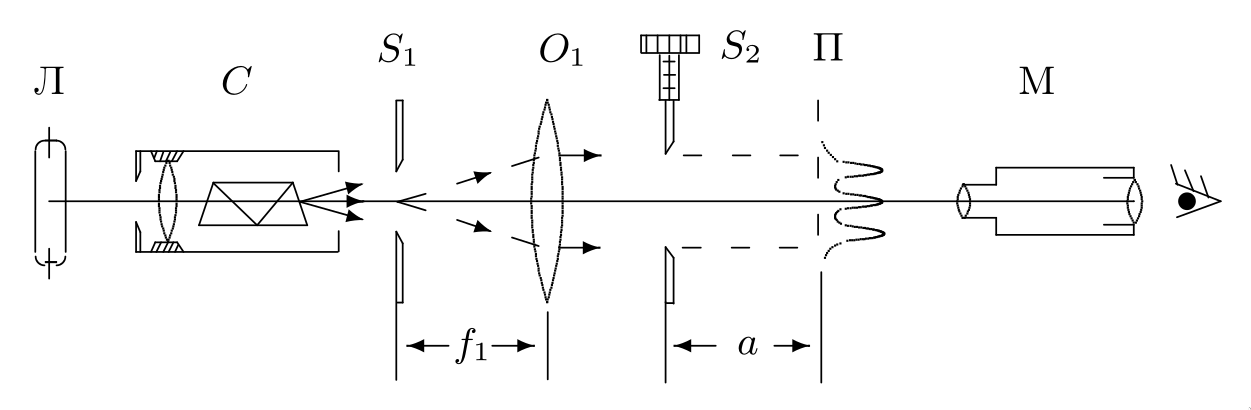
\includegraphics[scale=0.3]{lab_1.png}
    \caption{Схема установки для изучения дифракции Френеля}
\end{figure}

\noindent
Будем медленно придвигать микроскоп и снимать его координату, когда  меняется количество видимых темных полос. Также посчитаем по формуле (1) величину $2z_n$. Результаты занесем в табл. 1. Во время этих ихмерений ширина щели, измеренная микрометрическоим винтом, равна 0.21 мм.

\begin{table}[H]
    \centering
    \caption{Дифракция Френеля}
    \begin{tabular}{|c|c|c|} \hline
        $n$ & $x_n$, см & $2z_n$, мм \\ \hline
        1 & 46.3 & 0.20 \\ \hline
        2 & 46.2 & 0.19 \\ \hline
        3 & 46.0 & 0.21 \\ \hline
        4 & 45.8 & 0.21 \\ \hline
        5 & 44.4 & 0.23 \\ \hline
    \end{tabular}
\end{table}

\begin{figure}[H]
    \centering
    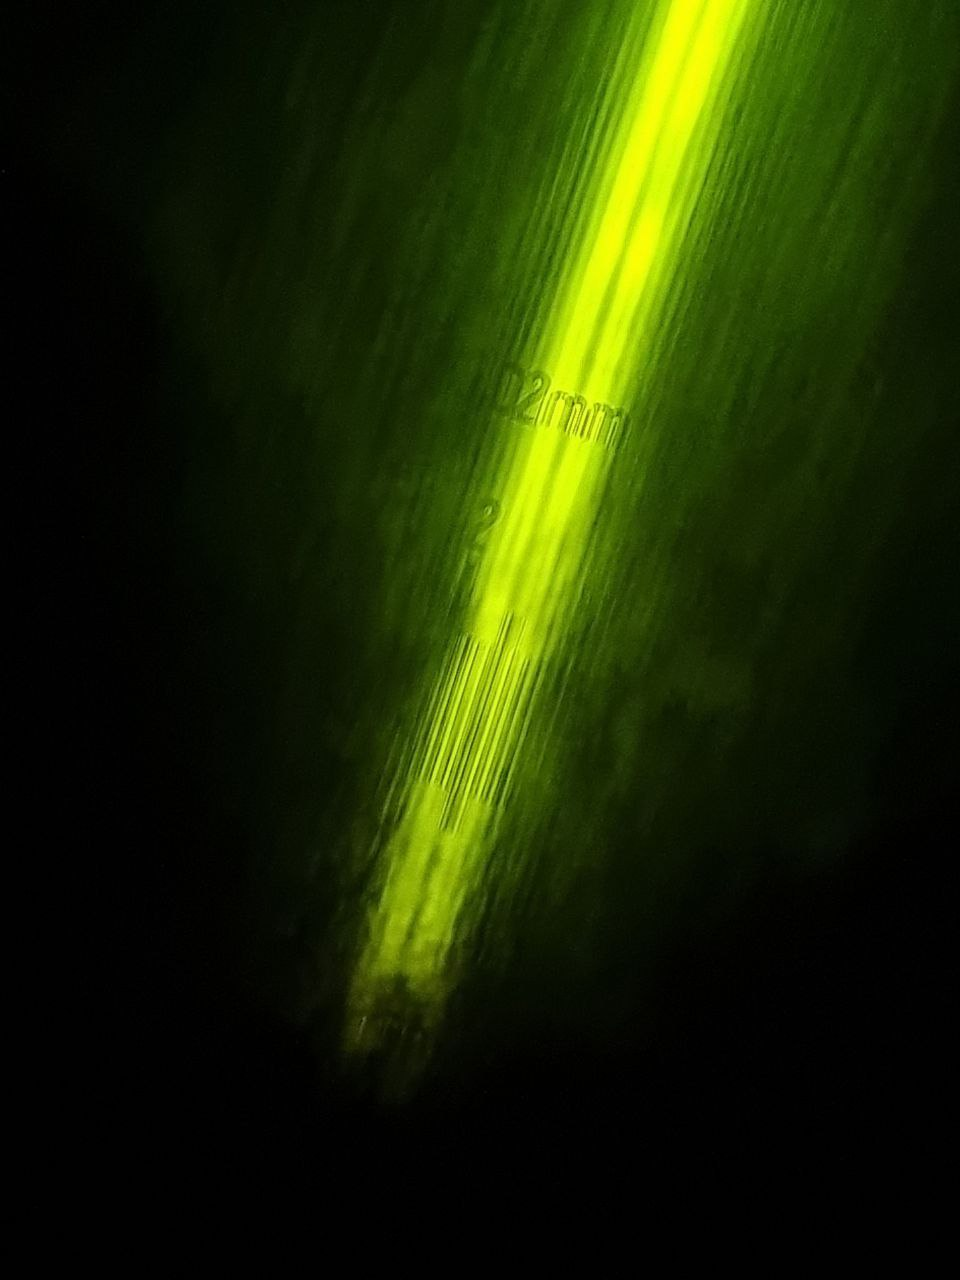
\includegraphics[scale=0.2]{pic_1.png}
    \caption{Наблюдение дифракции Френеля}
\end{figure}

\noindent
Построим теперь по табл. 1 график зависимости $2z_n$ от $n$, отложив на нем также ширину щели, измеренную непосредственно.

\begin{figure}[H]
    \centering
    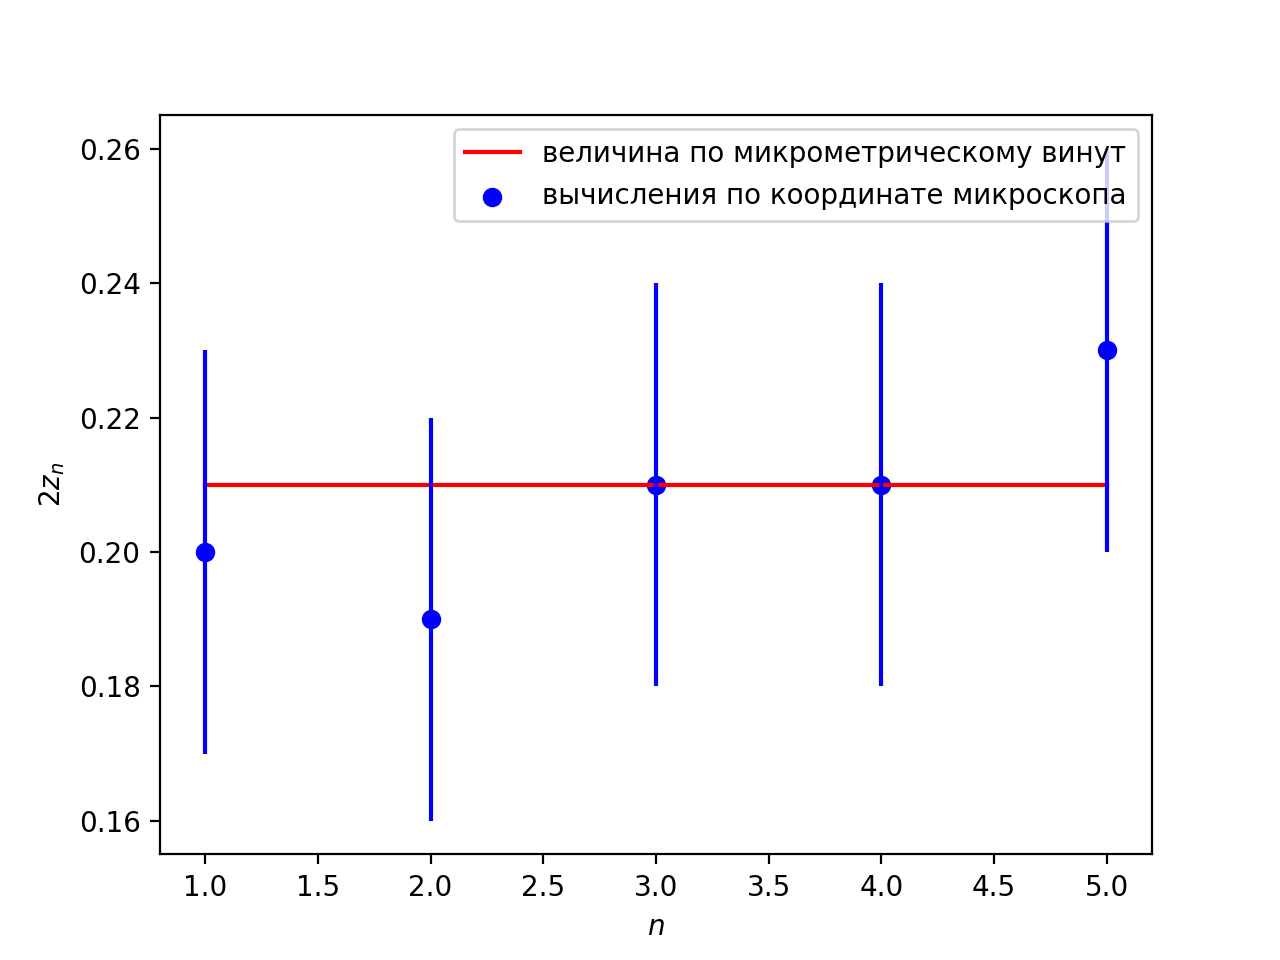
\includegraphics[scale=0.9]{1.png}
    \caption{Зависимость $2z_n$ от $n$}
\end{figure}

\newpage
\noindent
Теперь проделаем качественные наблюдения: дифракция на краю экрана и дифркация на препятствии (рис. 4 и рис. 5) соответственно.

\begin{figure}[H]
    \centering
    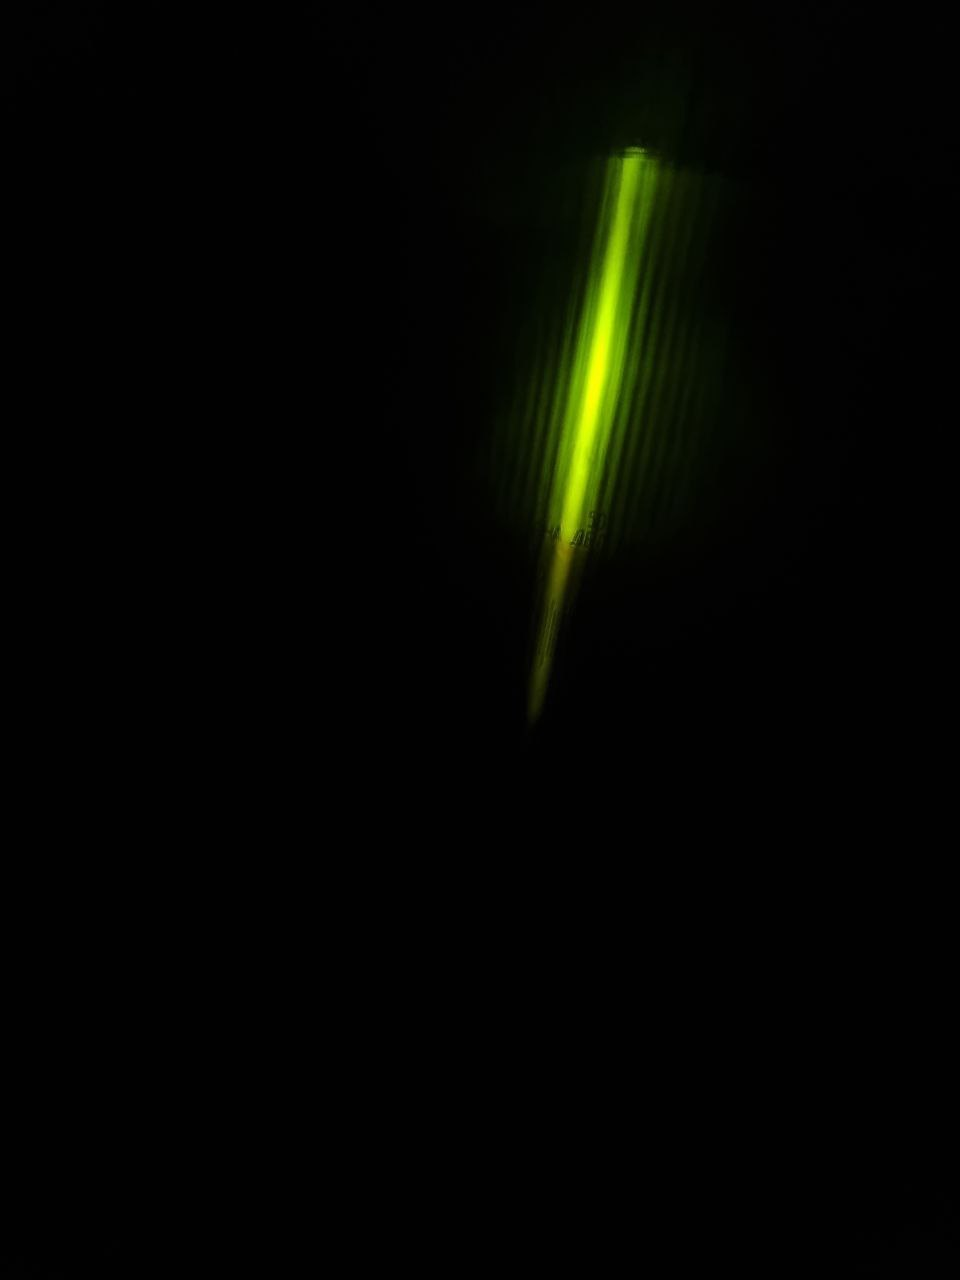
\includegraphics[scale=0.2]{pic_2.png}
    \caption{Дифракция на краю экрана}
\end{figure}

\begin{figure}[H]
    \centering
    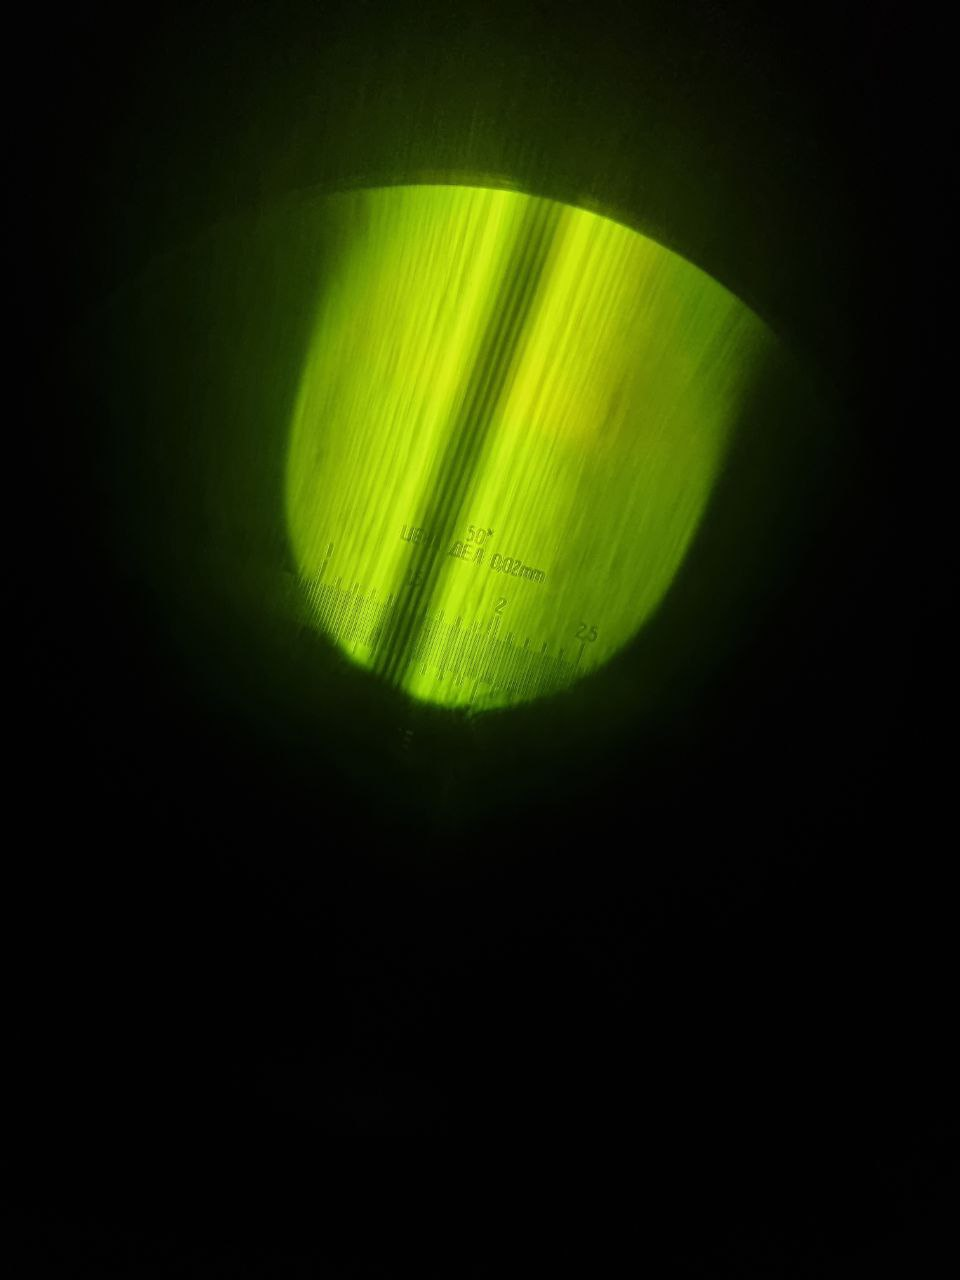
\includegraphics[scale=0.2]{pic_3.png}
    \caption{Дифракция на препятствии}
\end{figure}

\newpage
\paragraph{Дифракция Фраунгофера на щели} для иссладования дифракции Фраунгофера на щели соберем установку согласно схеме на рис. 6.

\begin{figure}[H]
    \centering
    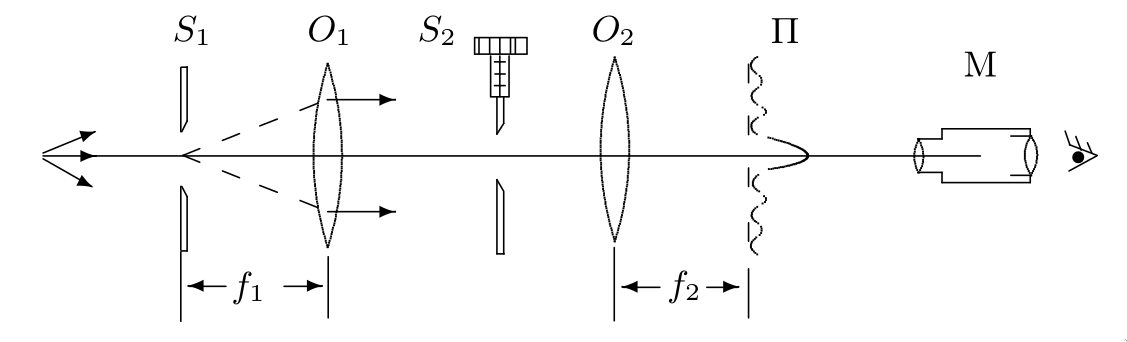
\includegraphics[scale=0.3]{lab_2.png}
    \caption{Схема установки для изучения дифракции Фраунгофера на щели}
\end{figure}

\noindent
Измерим координаты $X_m$ нескольких дифракционных миниммумов. Результаты занесем в табл. 2. По ней построим график на рис. 7.

\begin{table}[H]
    \centering
    \caption{Дифракция Фраунгофера на щели}
    \begin{tabular}{|c|c|c|c|c|c|c|c|} \hline
        $m$ & -3 & -2 & -1 & 0 & 1 & 2 & 3 \\ \hline
        $X_m$, мм & 1.05 & 1.16 & 1.30 & 1.43 & 1.55 & 1.68 & 1.78 \\ \hline 
    \end{tabular}
\end{table}

\begin{figure}[H]
    \centering
    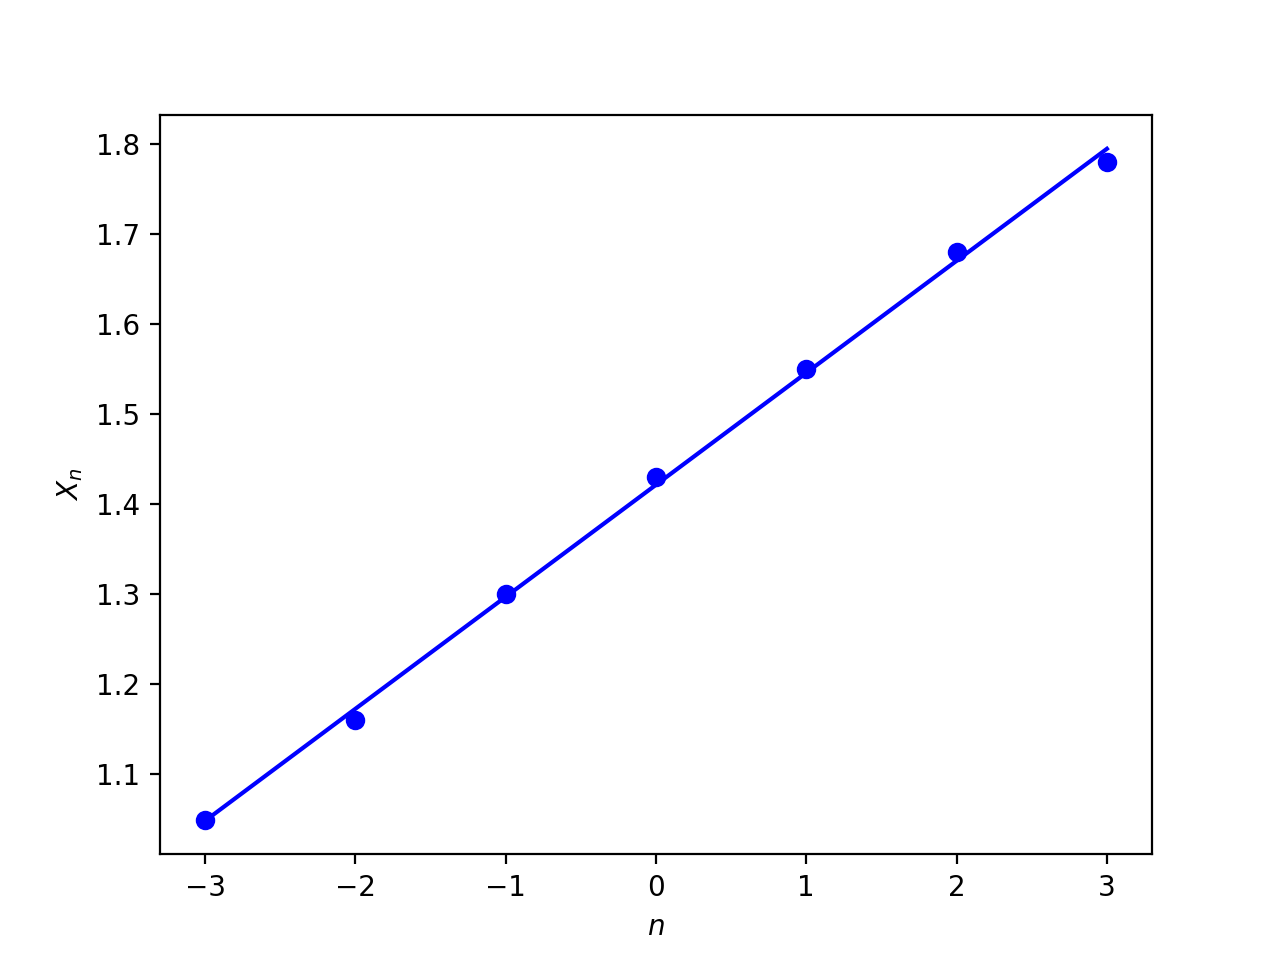
\includegraphics[scale=0.9]{2.png}
    \caption{Зависимость $X_n$ от $n$}
\end{figure}

\noindent
Из графика на рис. 7 и формулы (2) определим ширину щели $D = 0.22$ мм.

\begin{figure}[H]
    \centering
    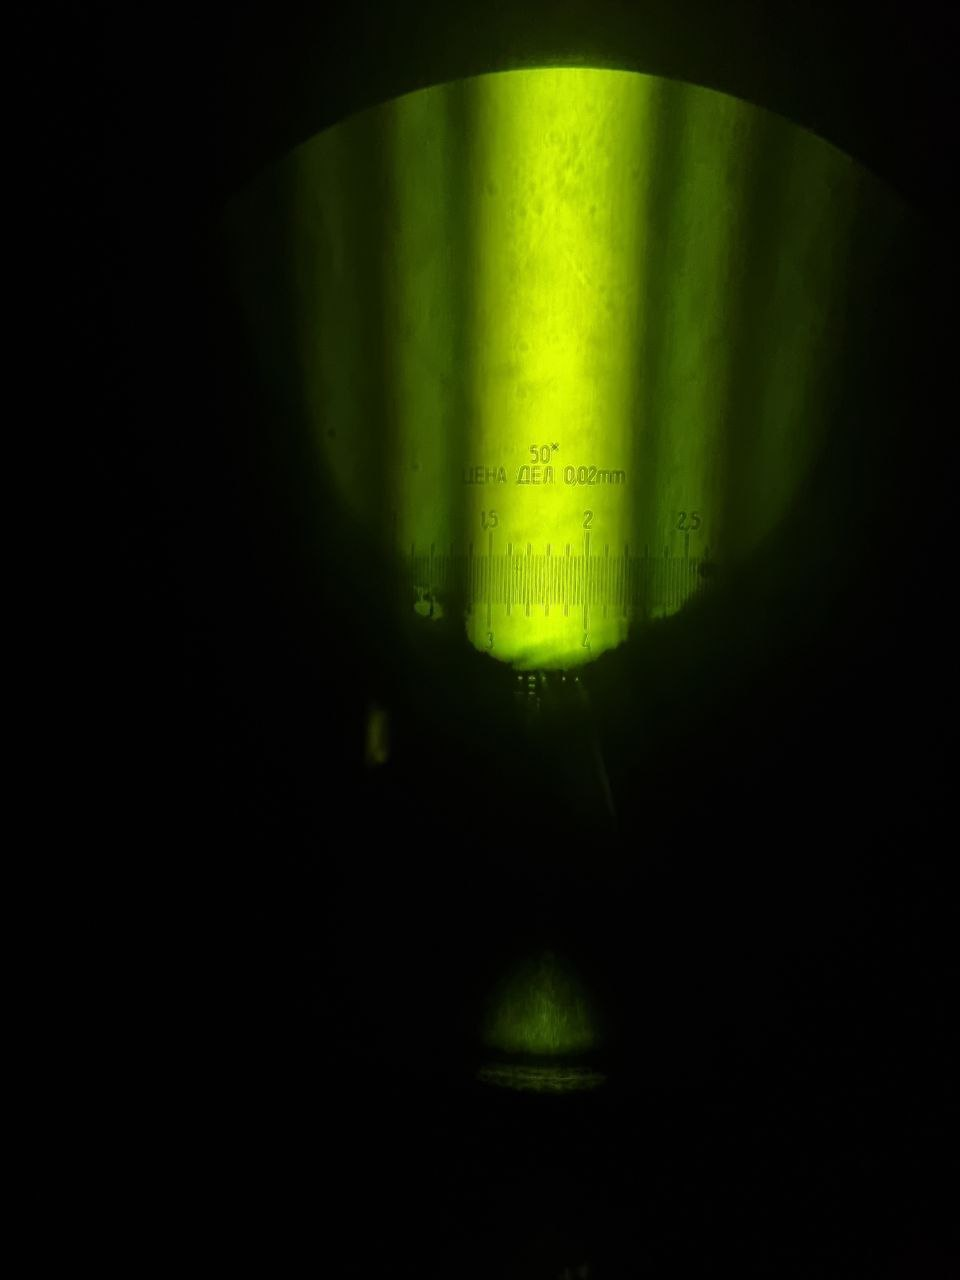
\includegraphics[scale=0.2]{pic_4.png}
    \caption{Дифракция Фраунгофера на щели}
\end{figure}

\paragraph{Дифракция Фраунгофера на двух щелях} для наблюдения дифракции Фраунгофера на двух щелях заменим в установке для дифракции Фраунгофера на одной щели щель $S_2$ на экран с двумя щелями Э. При этом фокусные расстояния линз равны $10.2$ см и $12.8$ см.

\begin{figure}[H]
    \centering
    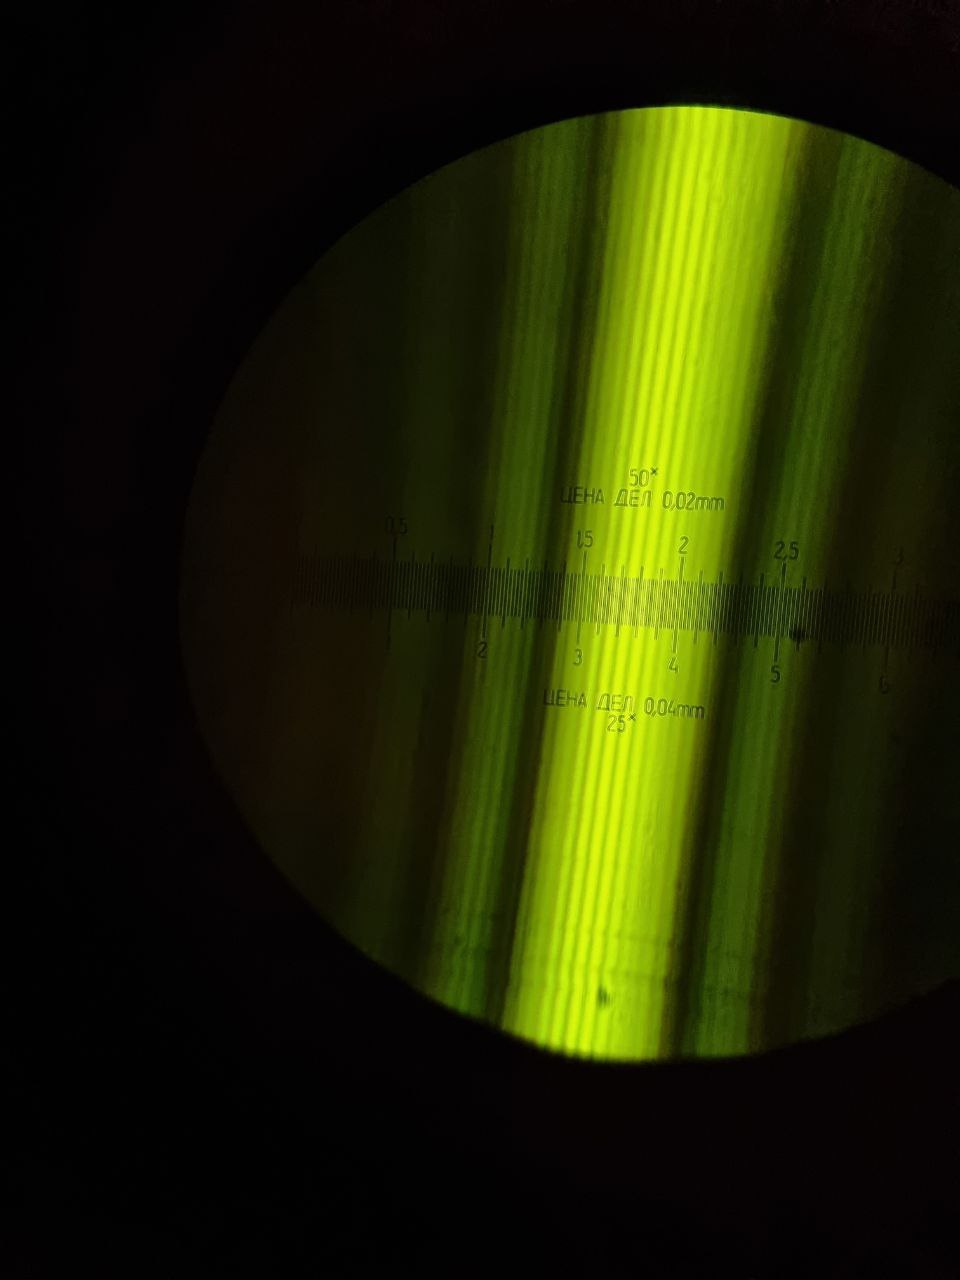
\includegraphics[scale=0.2]{pic_5.png}
    \caption{Дифракция Фраунгофера на двух щелях}
\end{figure}

\noindent
После получения четкой картины проводим измерения. Получаем, что первое исчезновение полос происходит при $b_0 = 0.14$ мм, ширина центрального максимума $X = 1.5$ мм, в нем находится $n = 15$ темных полос. Тогда $\delta x \approx \frac{X}{n} = 0.1$ мм и согласно формуле (3) $d = 0.69$ мм. Это значение близко к непосредственно измеренному $d = 0.72$ мм, хоть и несколько отличается от него. Тем не менее, точность можно считать приемлемой.

\paragraph{Влияние дифракции на разрешающую способность оптических приборов} для начала соберем установку согласно схеме на рис. 10.

\begin{figure}[H]
    \centering
    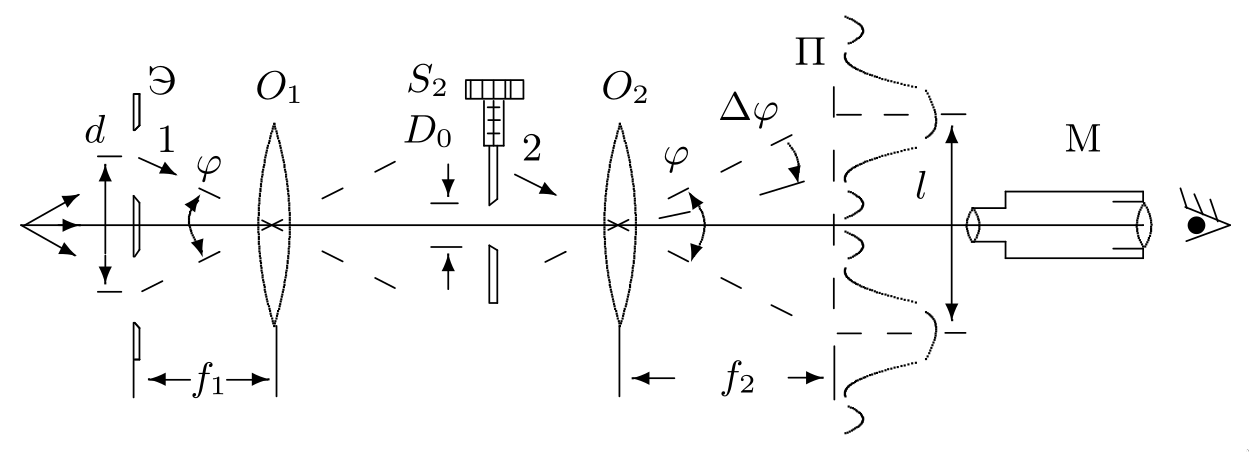
\includegraphics[scale=0.3]{lab_3.png}
    \caption{Схема установки для исследования влияния дифракции на разрешающую спосбоность}
\end{figure}

\noindent
Определим ширину щели $D_0$, когда изобаржения щелей становятся едва различимы: $D_0 = 0.32$ мм. Расстояние между щелями $d = 0.72$ мм, размеры щелей $0.32$ мм и $0.16$ мм. Оценим выполнимость криетрия Релея по формуле (4): $D_0 = 0.08$ мм. Это значение в 4 раза отличается от экспериментального значения $D_0$. Принимая в расчет оценочный характер измерений, а также то, что непонятно, когда считать щели различимыми, можем считать, что критерий Релея выполняется с приемлемой точностью.

\begin{figure}[H]
    \centering
    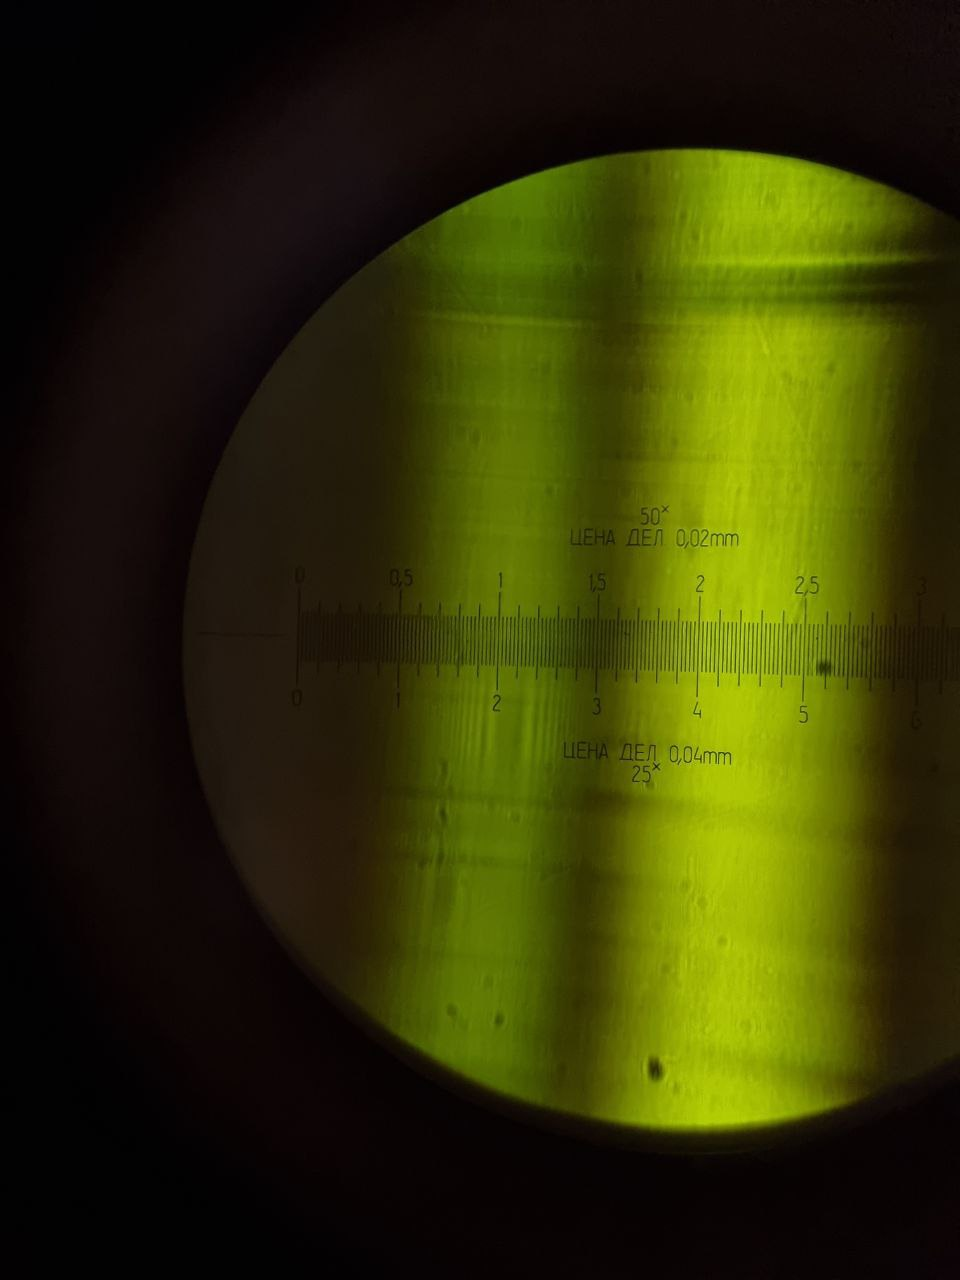
\includegraphics[scale=0.2]{pic_6.png}
    \caption{Изображения двух щелей при исследовании влияния дифракции на разрешающую способность}
\end{figure}

\section*{Вывод}
В работе была исследована дифракция Френеля, Фраунгофера на одной щели, Фраунговера на двух щелях. В опытах измерялась ширина щели и сравнивлась с реальной шириной, измеренной с помощью микрометричесокго винта. Также при исследованиии дифракции на двух щелях измерялось расстояние между ними. В каждом из опытов результаты измерений можно считать приемлемыми. Кроме того пронаблюдали явления дифракции на краю экрана и на препятствии (нити). \\
Оценили влияние дифракции на разрешающую способность оптического инструмента, убедились в применимости критерия Релея в данной ситуации. 

\end{document}

